\section{Factorization}
\subsection{Problem}
Given a number $N$, we have to find some factor of $N$.
\subsection{Classical Solution}
The classical solution requires to check if any number from $1$ to $\sqrt{N}$ divides $N$. So, in total we will be checking $\sqrt{N}
$numbers and hence the time complexity is $O(\sqrt{N})$.
\subsection{Quantum Solution}
For the quantum solution, we assume a specific class of $N$. First, it must not be a multiple of 2 which can be easily checked. Second, the number must not be of the form $a^b$ $\forall b\in \{2,3,4...\log N\}$. This can be easily checked in $O((\log N)^3)$ steps by computing $a$ for all values of $b$.\\
The algorithm first reduces the problem of factorization to order finding and then use the algorithm for order finding to find the factor. It uses the following theorem:\\
\\{\scshape Theorem 1: } Suppose $N$ is an $L$ bit composite number, and $x \leq N$ is a non-trivial solution of $x^2 = 1(\bmod N) $ then either $gcd(x-1,N)$ or $gcd(x+1,N)$ is a non-trivial factor of $N$.\\
\\{\scshape Theorem 2: } Suppose $N = p_1^{\alpha_1}p_2^{\alpha_2}...p_m^{\alpha_m}$ is the prime factorization such that all $p_i$ are odd i.e. $N$ is not even. Let $x$ be a randomly chosen number less than $N$ and co-prime to $N$ and let $r$ be the order of $x$ w.r.t $N$. Then, 
\begin{equation}
p(\text{r is even and $x^{r/2} \ne -1 (\bmod N)$ }) \geq  1- \frac{1}{2^m}
\end{equation}This probability is always greater than half and hence repeated application will take it close to 1. Combining all these facts, we can efficiently compute some factor of a given composite number.\\
\begin{figure}[h]
\centering
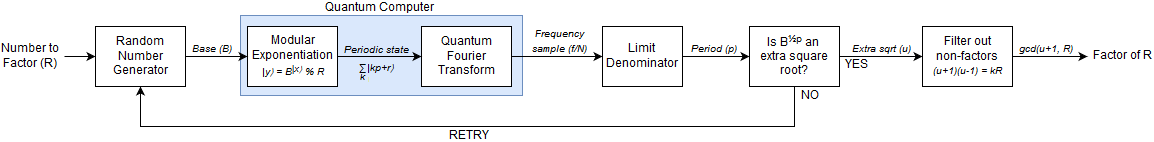
\includegraphics[width=1\textwidth]{images/factor.png}
\label{factor}
\caption{Circuit for finding a factor of a given number N}
\end{figure}

\begin{enumerate}
\item Ensure that $N$ is odd. If not then return $2$ as a factor. This can be done in $O(1)$ steps.
\item Ensure that $N$ is not of the form $a^b$ otherwise return $a$. This can be done in $O(L^3)$ steps.
\item Randomly choose a number $x \in \{0,1,2...N-1\}$. If $x$ is not co-prime to $N$, then return $gcd(x,N)$ as  a factor. 
\item Since $x$ is co-prime to $N$, there would exist an order of $x$ w.r.t. $N$ say $r$. Compute thus $r$ using the order finding circuit.
\item If r is even and $x^{r/2} \ne -1 (\bmod N)$ then compute $gcd(x^{r/2}-1,N)$ and $gcd(x^{r/2}+1,N)$. If either one of them is a non-trivial factor, return it. Otherwise, the algorithm failed and repeat for a different value of $x$.
\end{enumerate}
In all, we require $O(L^3)$ operations to calculate a factor of  the number $N$.\\
hence we have found a way to calculate the factors of a given number $N$. The inability of computing such factorization for large numbers is one of the key points in the modern cryptosystems like RSA. If a quantum computer is built which is able to perform the above algorithm, these systems will be broken. hence quantum computer poses a great threat to our privacy until we find some other stronger system.

